%\begingroup Introduction

\section{Introduction}

For many years, database research focused primarily on relational databases, which organize data into tables with fixed schemas~\citep{DBLP:persons/Codd71a}. The rise of \acrshort{nosql} databases in the early 2000s popularized additional data models and formats, including document, graph, key-value, and wide-column data~\citep{PolyglotPersistance}.

These models are well suited to different types of applications and workloads. They also introduce a new difficulty: moving data between systems that use different models is considerably more complex and error-prone than migrating data between relational databases. Moreover, the \acrshort{nosql} ecosystem still lacks unified theoretical foundations, common standards, and tools for managing data across models.~\citep{CSUR-Jiaheng}

\begin{example}
\label{ex:mm-data}
The \emph{Yelp Academic Dataset} contains JSON collections describing businesses, users, reviews, tips, friendships, check-ins, and photos. We use a subset of this dataset in which the \code{user} data is represented as a relational table, \code{business} as a document collection, \code{FRIEND} as a graph relationship, and \code{review} as a wide-column family. The representations remain connected through shared identifiers, which allows results from different models to be combined. The resulting multi-model representation is shown in \Cref{fig:mm-data}.
\end{example}

\begin{figure}[ht]
    \centering
    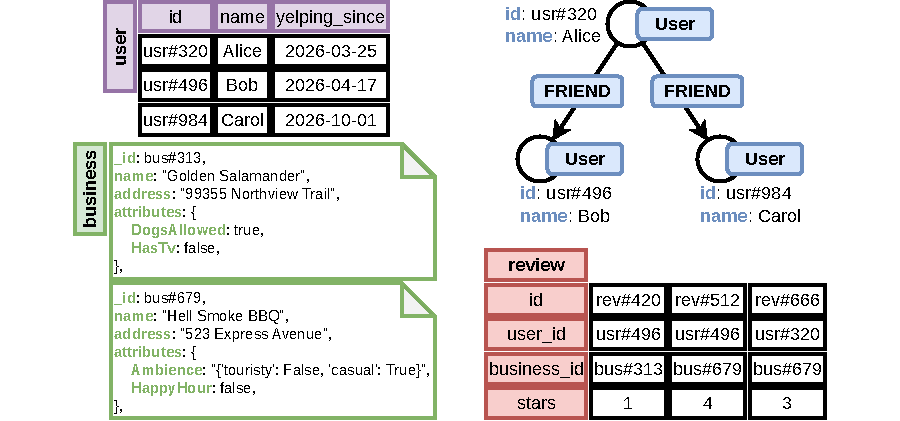
\includegraphics[width=\textwidth]{img/commentary-mm_data.pdf}
    \caption{Multi-model representation from \Cref{ex:mm-data}: a subset of the Yelp Academic Dataset represented in multiple data models and connected through shared identifiers.}
    \label{fig:mm-data}
\end{figure}

Each model offers a different advantage. Relational data is suitable for structured data with fixed schemas, documents naturally represent semi-structured and nested data, graphs support queries over connectivity, and wide-column stores are optimized for high-throughput workloads. The same specialization makes cross-model use difficult: combining results from several databases is not straightforward and can introduce semantic inconsistencies if done incorrectly.

This setting is commonly called \term{multi-model data}. Using a separate database system for each model is known as \term{polyglot persistence}~\citep{PolyglotPersistance}. \term{Polystores} provide a unified interface over several databases~\citep{9252014}, while \term{multi-model databases} combine several models within one system~\citep{CSUR-Jiaheng}. Both approaches still have to address the heterogeneity of the underlying models and systems; moreover, no multi-model database currently supports all commonly used data models~\citep{DBEngines2026}. These challenges motivated us to develop a unified approach to multi-model data management, presented on the following pages.

This report follows the same structure as the thesis itself:
\begin{itemize}
    \item The \emph{Vision} section formulates the research goals and the challenges of multi-model data management.
    \item The \emph{Foundations} section introduces the common terminology and summarizes our previous work on modeling, transformations, inference, and querying.
    \item \emph{Evolution Management} describes the propagation of schema changes to logical schemas, data, and queries.
    \item \emph{Self-Adaptation} considers workload-aware optimization over alternative multi-model configurations.
    \item \emph{Complementary Approaches} presents benchmark generation and schema-free query unification, both of which provide additional support for the main research direction.
\end{itemize}

%\endgroup
%\begingroup Vision

\section{Vision}

When it comes to data, our primary goal is to extract information from it by asking questions and obtaining answers, in a process commonly known as \term{querying}. For multi-model data, querying crosses the boundaries of different models and, in the case of polyglot persistence, different database systems as well.

Querying requires several supporting capabilities. We need to \term{model} data so that we can reason about its structure and semantics, and in some cases we need to \term{infer} the schema from existing data. Modeling and inference are closely related to \term{evolution}: when a schema changes, we must propagate the change to the data and to the queries that depend on it. In a multi-model setting, this may also require us to \term{transform} data between different models.

Although our main concern is correctness, it is not the only one. The system should also query data efficiently and should be able to select an appropriate combination of models for a given workload. Because doing so manually is difficult, we want the system to adapt its internal representation through \term{self-adaptation}.

This vision, introduced in \paperRef{vldb_2024}, combines modeling, inference, transformation, querying, evolution, and optimization within one multi-model data management framework~\citep{ideas2022vision, Jiaheng2023Survey}.

\subsection{Level of Automation}

We introduce automation gradually, distinguishing three levels according to the primary actor, that is, the main source of decisions and changes~\citep{ideas2022vision}:
\begin{itemize}
    \item \term{User-driven} -- users explicitly \emph{model} the data, create \emph{queries}, \emph{transform} the data, and \emph{evolve} the schema; the system propagates the changes to the data and queries.
    \item \term{Data-driven} -- the system \emph{infers} the schema from the data and updates it when the structure of the data changes.
    \item \term{System-driven} -- the system uses \emph{self-adaptation} to analyze the workload and data characteristics and proactively \emph{transforms} the data into a configuration suitable for the current workload.
\end{itemize}
These levels are not strictly disjoint; they describe the dominant source of decisions and control. More automation reduces manual work and can reveal solutions that would be difficult to find manually, but it also increases system complexity and may reduce the user's control over the process.

\subsection{Challenges}

The heterogeneity of the participating models is the main source of complexity \citep{Jiaheng2023Survey}. Document, wide-column, and key-value models are often aggregate-oriented, while relational and graph models tend to decompose data into records connected by references or relationships. Some models are schema-less or only partially schema-full, whereas relational models generally require a fixed schema. These differences also affect query languages, integrity assumptions, and optimization techniques. There is consequently no one-size-fits-all solution: the best representation depends on the data, the workload, and the capabilities of the underlying systems.

Classical conceptual modeling approaches such as \acrshort{er} and \acrshort{uml} provide useful technology-independent descriptions of a domain, but they do not by themselves provide mappings, transformations, and query execution across heterogeneous models~\citep{ER, UML}. Similarly, polystore and multistore systems combine existing database technologies but must still manage the semantic relationships between their representations. Our vision treats conceptual modeling as the semantic basis for these broader operations.

\subsection{Previous Work}
\label{sec:previous-work}

The research presented in this thesis is based on a previous line of work on modeling~\citep{mm_cat, mm_cat_journal}, querying~\citep{mm_quecat, koupil2023universal}, and inference~\citep{mm_infer, koupil2022mminfer} of multi-model data. In the following sections, we will use \uv{we} and \uv{our} to reference the previous work of our research group on these topics.

Other topics, i.e., evolution, self-adaptation, benchmarking, and schema-free query unification, are novel contributions of this thesis.

\subsection{Research Questions}

We formulate the vision as concrete research questions. Our previous work already addressed some of them:
\begin{itemize}
    \item \term{Modeling} -- How can heterogeneous data models be represented in a common semantic framework without erasing their model-specific structure?
    \item \term{Transformations} -- How can data be transformed between different models without the need to write custom transformation rules for each pair of models?
    \item \term{Querying} -- How can queries be unified across different data models, supporting a common, practically useful subset of features of each model, and allowing for cross-model queries and optimizations?
\end{itemize}
We use these answers as a foundation for the rest of our research. In this thesis, we address the following questions:
\begin{itemize}
    \item \term{Evolution} -- How can changes be propagated across conceptual and logical schemas, data, and queries in a multi-model environment? How can uncertain or ambiguous evolution decisions be supported by data-derived semantic evidence?
    \item \term{Self-adaptation} -- How can a multi-model system choose suitable representations for a workload without exhaustively materializing and benchmarking all alternatives?
    \item \term{Benchmarking} -- How can such systems be evaluated when real multi-model benchmarks and workloads are scarce?
    \item \term{Schema-free Query Unification} -- How can multi-model queries be unified when a shared conceptual schema is unavailable?
\end{itemize}

%\endgroup
%\begingroup Foundations

\section{Foundations}

The preexisting work, mentioned in \Cref{sec:previous-work}, is based on category theory. It provides a formal framework for modeling, transformations, inference, and querying of multi-model data, allowing us to unify these operations for different data models and database systems.

\subsection{Common Terminology}

We distinguish three abstraction levels commonly used in database design: \term{conceptual}, \term{logical}, and \term{physical}. A conceptual schema is a \emph{platform-independent} description of the domain. It captures concepts and their relationships without committing to a particular database technology. A logical schema is \emph{platform-specific}---it describes how selected parts of the conceptual schema are represented in a concrete data model. Finally, a physical schema describes the data structures used to store the data and implement indexes. We focus primarily on the conceptual and logical levels, but consider physical aspects when they affect the overall approach.

This separation allows us to map one conceptual schema to several logical representations. The mappings preserve the semantics of the domain while allowing each database to use the structures and operations native to its model.

Each data model has its own terminology, so we define model-agnostic terms:
\begin{itemize}
    \item At the logical level, a \term{kind} is a class of items, such as a relational table, a document collection, or a collection of nodes or edges with the same label. An \term{attribute} is a field of a kind, such as a table column, document field, or node property.
    \item At the physical level, a \term{record} is an item of a kind, and a \term{value} is the value of an attribute in a record.
    \item At the conceptual level, a \term{simple type} is a value-carrying element (e.g., id, name), while a \term{complex type} is a structure consisting of simple types (e.g., user, business). A \term{projection} is a directed connection from a complex type to another simple or complex type (e.g., a user has a name). The \term{properties} {[}of a complex type{]} are all the simple types connected to it by a projection.
\end{itemize}
These terms abstract away model-specific details while preserving the structure needed for querying, transformation, and evolution.

\subsection{Category Theory}

Category theory provides the formal language for describing the structures and relationships in our approach. A \term{small category} $\mathcal{C} = (\mathcal{O}, \mathcal{M}, \circ)$ consists of a set of \term{objects} $\mathcal{O}$, a set of \term{morphisms} $\mathcal{M}$, and a composition operation $\circ$ over morphisms. A morphism $f \in \mathcal{M}$ is a directed connection between two objects $A, B \in \mathcal{O}$, denoted $f : A \to B$. For each object $A \in \mathcal{O}$, there is an \term{identity morphism} $1_A : A \to A$. Finally, the composition operation $\circ$ is associative and has the identity morphisms as its neutral elements.

Another important concept in category theory is a \term{functor} which maps objects and morphisms between categories while preserving identities and composition.

In our setting, a conceptual schema is a small category called a \term{schema category}. Its objects represent simple and complex types, and its morphisms represent projections between them. The category therefore captures both the domain concepts and the paths through which they are related. A logical schema is also a schema category, but its objects and morphisms have the specific semantics of the underlying data model.

The schema category introduced in \Cref{ex:schema-category} is used throughout the report. The ovals represent conceptual objects, while the arrows represent projections. This category is not merely a diagram of the domain: it provides the structure against which mappings, query patterns, and schema modifications can be defined.

\begin{example}
\label{ex:schema-category}
The schema category for the multi-model representation from \Cref{ex:mm-data}, depicted in \Cref{fig:schema-category}, contains objects for types such as \object{User}, \object{Review}, and \object{Business}, as well as their simple properties. Its morphisms represent projections such as the connection from \object{Review} to its identifier and the relationship between a review and a business. Each morphism is identified by a numeric \term{signature}.
\end{example}

\begin{figure}[ht]
    \centering
    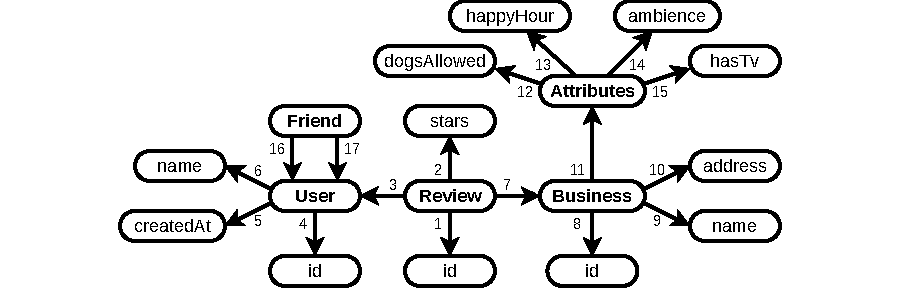
\includegraphics[width=\textwidth]{img/commentary-schema_category.pdf}
    \caption{Schema category from \Cref{ex:schema-category}, modeling the data from \Cref{fig:mm-data}. The objects represent conceptual types and the morphisms represent projections between them.}
    \label{fig:schema-category}
\end{figure}

Each logical schema must conform to the constraints of its data model. A relational schema is flat, whereas a document schema can express nested structures. The logical schema is connected to the conceptual schema by a \term{mapping}, which is a functor from the logical category to the conceptual category. This mapping preserves the semantics of the conceptual schema while allowing the logical representation to use model-specific structures, tailoring each logical schema to the capabilities of its underlying model.

\begin{example}
\label{ex:mapping}
The mapping in \Cref{fig:mapping} illustrates how the conceptual structure can be realized differently. The wide-column model cannot store the complex \object{User} type as a nested column, but it can embed the simple type \object{id} into \object{review} as \object{user\_id}. The corresponding composite morphism \signature{3.4} represents the path through \object{Review} and \object{User} via morphisms \signature{3} and \signature{4}.
\end{example}

\begin{figure}[ht]
    \centering
    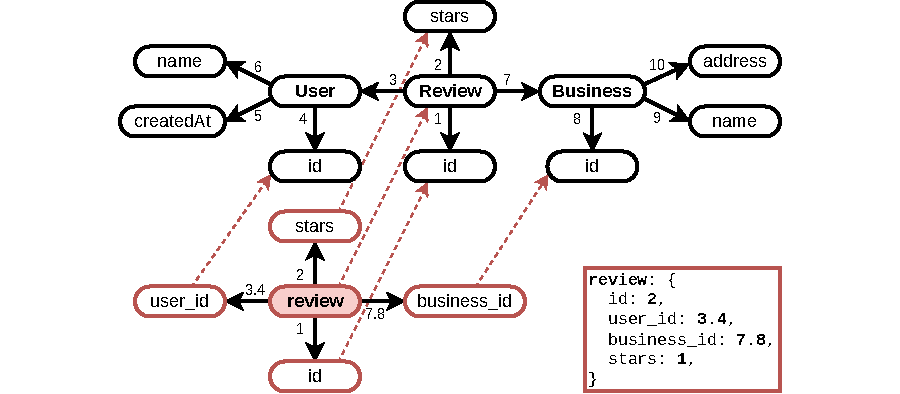
\includegraphics[width=\textwidth]{img/commentary-mapping.pdf}
    \caption{Mapping from \Cref{ex:mapping} between a wide-column logical schema and the conceptual schema from \Cref{fig:schema-category}. The logical representation adapts the conceptual structure to the capabilities of the underlying model.}
    \label{fig:mapping}
\end{figure}

\subsection{Modeling, Transformations, and Querying}

Our previous work introduced an \term{instance category} with the same structure as the schema category and algorithms for converting data between databases and instance categories~\citep{mm_cat, mm_cat_journal}. This common representation allows us to transform data between supported models without defining a separate transformation for every pair of models. Database-specific wrappers provide the concrete data structures and the required \acrshort{ddl} and \acrshort{dml} statements, while the transformation algorithms remain model-independent~\citep{mm_cat_journal}.

Querying heterogeneous data is difficult because each database system has its own language, and because systems using the same model may still differ in syntax and semantics~\citep{Jiaheng2023Survey}. Existing extensions such as \acrshort{sql}/JSON~\citep{SQLJSON} and \acrshort{sql}/PGQ~\citep{SQLPGQ} cover particular combinations of models, but do not provide a general solution for cross-model queries. In a polyglot persistence system, users would otherwise have to write several native queries and combine their results manually.

These requirements led us to develop the \term{multi-model query language} (\term{\acrshort{mmql}})~\citep{mm_quecat, koupil2023universal}. \acrshort{mmql} is defined over the schema category and is therefore independent of the underlying models and database systems. During execution, the query engine matches query patterns against the available logical schemas, splits a query into maximal subqueries executable by individual databases, translates them into native languages, executes them, and combines the results.

\begin{example}
\label{ex:query-multi}
Consider the query: \emph{Find all reviews with at least 3 stars about a business with id \code{bus\#679}, ordered by the number of stars (ascending). For each review, return the stars and the author's name.} No single logical schema contains all required information, so \acrshort{mmql} splits the query into subqueries over the wide-column and relational databases and joins their results using the shared \object{User} identifier.
\end{example}

\begin{figure}[ht]
    \centering
    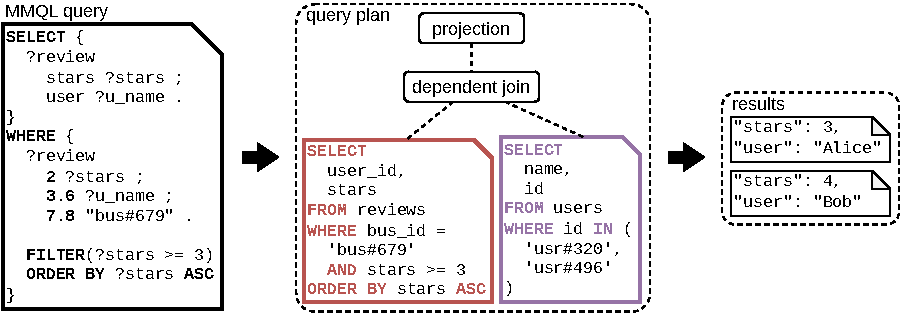
\includegraphics[width=\textwidth]{img/commentary-query_multi.pdf}
    \caption{Multi-model query from \Cref{ex:query-multi}. The query is split into subqueries executed in different databases and then combined according to the shared conceptual schema.}
    \label{fig:query-multi}
\end{figure}

Because redundancy may make several query plans possible, the engine estimates their cost and selects the best one. We extended the query engine with predicate pushdown, dependent joins, and cache-based cost estimation~\citep{strobl_2026} (under review). The same conceptual representation therefore supports not only a unified interface, but also cross-model query planning and optimization. These optimizations are contributions of this thesis, rather than part of the previous modeling and querying work.

\subsection{Related Work}

Traditional conceptual modeling approaches such as \acrshort{er}~\citep{ER} and \acrshort{uml}~\citep{UML} were designed primarily for relational or relational-like data. They do not directly capture the structures of some \acrshort{nosql} models or the relationships between several models and database systems. We use them as inspiration for the conceptual level, but we represent the conceptual schema as a category so that the same structure can also support mappings, transformations, evolution, and cross-model querying.

The closest practical line of work includes \term{U-schema}~\citep{DBLP:journals/is/CandelRM22} and its extensions, such as \term{Orion}~\citep{DBLP:conf/er/ChillonRM21a, 10.1109/TKDE.2024.3362273} and \term{SkiQL}~\citep{skiql}. These approaches primarily unify data at the logical level. A single logical schema may fail to express the features of all underlying models, while several disconnected logical schemas introduce redundancy and make their semantic relationships less explicit. Our approach retains one platform-independent conceptual schema and connects it to specialized logical schemas through mappings. This allows each database to use a suitable representation while preserving a shared semantic view. SkiQL also differs in its purpose: it queries schema structure, whereas \acrshort{mmql} queries data content over the conceptual schema.

Category theory has also been used to formalize heterogeneous data management and transformations~\citep{DBLP:journals/corr/abs-2201-04905, lu2025part1, lu2025part2}. These works provide rigorous categorical algebra and calculus for multi-model predicates, allowing us to model the multi-model data. Our approach has a broader scope---it uses category theory to support the full set of above-described operations. We also implement these operations over practical database systems to validate and evaluate the approach.

Finally, polystore and mediator-style systems provide unified access to heterogeneous backends~\citep{conf/cikm/LuHC18, DBLP:journals/ijcc/BondiombouyV16, alotaibi2020estocada}. Multi-model databases and standards such as \acrshort{sql}/XML, \acrshort{sql}/JSON, and \acrshort{sql}/PGQ extend individual systems or languages to additional models~\citep{Jiaheng2023Survey, SQLXML, SQLJSON, SQLPGQ}. These approaches demonstrate the value of interoperability, but generally treat local representations as given. Our framework combines the conceptual schema, logical representations, mappings, and queries in one foundation, which lets us reason about both interoperability and the choice of representation itself.

%\endgroup
%\begingroup Evolution

\section{Evolution Management}

Everything is subject to change, and multi-model data is no exception. Changes may occur in the conceptual or logical schema, in the data itself, or in the queries defined over the data. \term{Evolution management} involves detecting these changes, describing them formally, and propagating them to all affected components so that the system remains consistent and correct. This is especially challenging in a multi-model environment, where the relationships between components are complex and a local change can have consequences throughout the system.

The main challenges are to describe and propagate changes independently of the underlying data models, to provide an evolution language that captures both atomic operations and higher-level intent, and to propagate changes to data and queries. The system should also detect changes originating in the data, choose between alternative migration and synchronization strategies, and request user input only when the available information is insufficient for a reliable decision.

\subsection{Evolution Hierarchy}

Our approach starts with a hierarchy of components and rules for propagating changes between them. The conceptual schema is at the top of the hierarchy and can be modified through atomic \emph{schema modification operations} (\acrshort{smo}s). These operations may be provided by the user or inferred from changes in the data. Changes to the conceptual schema are propagated to the logical schemas, and changes to the logical schemas are propagated to the data through \acrshort{ddl} and \acrshort{dml} statements.

Queries are defined over the conceptual schema and translated into native database queries only at execution time. Consequently, changes to logical schemas do not directly affect \acrshort{mmql} queries; queries are updated when the conceptual \acrshort{smo}s affect their selection or projection patterns.

Propagation can also proceed bottom-up: the system may observe a change in the data, infer the corresponding conceptual operation, and then apply the usual top-down propagation. Changes in the workload may trigger self-adaptation and lead to changes in logical schemas and data layouts. The resulting hierarchy is shown in \Cref{fig:evolution}.

\subsubsection{Schema Modification Operations}

The \acrshort{smo}s were proposed in \paperRef{cikm_2022} and formally defined in \paperRef{rcis_2025}. We divide them into three groups:
\begin{itemize}
    \item \term{basic} operations work with individual objects and morphisms, such as \code{create}, \code{delete}, and \code{move},
    \item \term{composite} operations capture frequent higher-level patterns, such as properties, relationships, arrays, sets, and maps (e.g., \code{createProperty}),
    \item \term{complex} operations capture larger restructurings, such as \code{group}, \code{join}, and \code{asMap}.
\end{itemize}
Users can therefore express changes at an appropriate level, while the system can reduce every operation to basic operations with explicit preconditions and postconditions. This makes propagation analyzable and allows the system to optimize, roll back, or postpone individual steps. We also distinguish between \term{light} changes, which update the conceptual schema and mappings but leave logical schemas and data unchanged, and \term{heavy} changes, which propagate to the logical schemas and data as well.

\begin{figure}[ht]
    \centering
    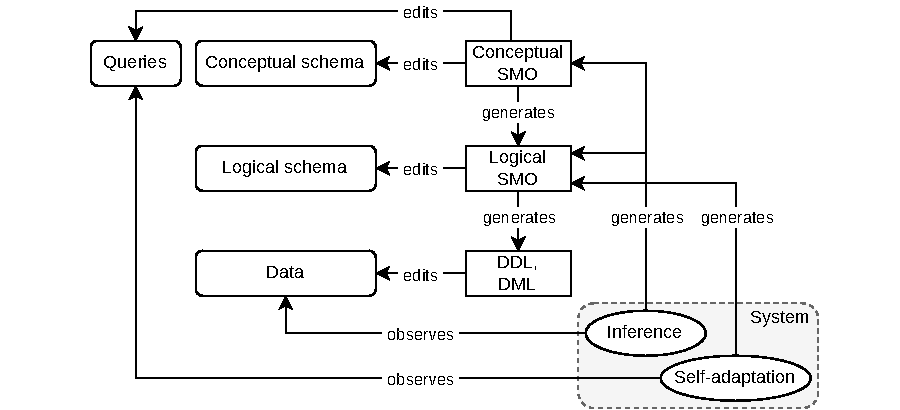
\includegraphics[width=\textwidth]{img/commentary-evolution_hierarchy.pdf}
    \caption{Hierarchy of components for evolution management. Changes are propagated downward from the conceptual schema, while changes originating in data or query workloads can be observed and propagated upward by inferring the corresponding operations.}
    \label{fig:evolution}
\end{figure}

\subsubsection{Propagation to Data and Queries}

The propagation to queries builds on the approach from \paperRef{edbt_2024}. Each query is analyzed through its selection and projection categories, and the system evaluates how a basic \acrshort{smo} affects these categories and clauses such as \code{FILTER}, \code{DISTINCT}, \code{ORDER BY}, and aggregations. Some changes preserve the query behavior, some require a restricted rewrite, and some are too destructive to repair automatically.

The difficult cases are those in which the change decreases the available information, for example by deleting a property used by an existing query. The system may then reconstruct the missing values using a phantom representation, replace them using functional dependencies, or ask the user for additional guidance. \term{FDepHunter}, described in \paperRef{vldb_2025_fdephunter}, provides semantic evidence for choosing between these alternatives by discovering and refining functional dependencies in real data.

\begin{figure}[ht]
    \centering
    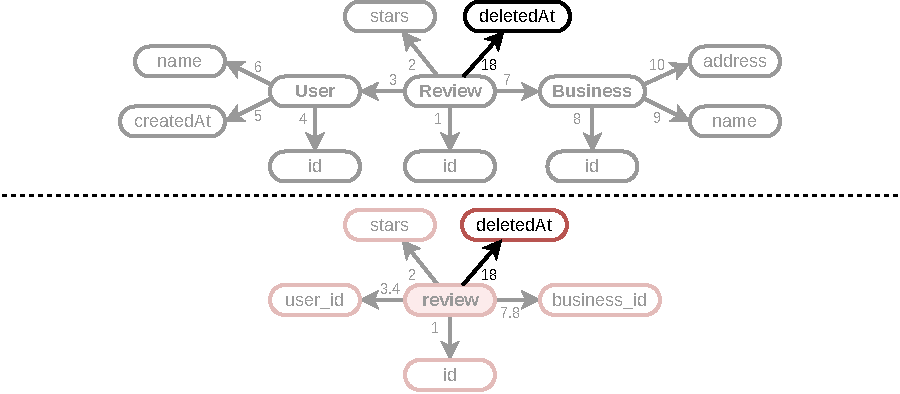
\includegraphics[width=\textwidth]{img/commentary-evolution_add.pdf}
    \caption{Propagation from \Cref{ex:evolution-add}: adding a property to the conceptual schema and propagating the change to a logical schema through schema modification operations.}
    \label{fig:evolution-add}
\end{figure}

\begin{example}
\label{ex:evolution-add}
Starting with the conceptual schema and the wide-column logical schema, users can apply \code{createProperty} to add \object{deletedAt} to \object{Review}. As shown in \Cref{fig:evolution-add}, the system updates the mapping and adds the corresponding attribute to the logical schema and data. Because the existing query does not use this property, it remains unchanged; users may nevertheless add the property later to filter out deleted reviews. More complex operations, such as converting the properties of \object{Attributes} into a key-value map, may require a query rewrite.
\end{example}

\subsection{Level of Automation}

We distinguish three levels of automation according to how much of the propagation process the system determines and executes~\citep{ideas2022vision}:
\begin{itemize}
    \item \term{Rule-based adaptation} -- the user or change-detection mechanism specifies what should change, and the system deterministically executes how it is propagated.
    \item \term{Learning-based adaptation} -- the system chooses among several admissible propagation or synchronization strategies.
    \item \term{Self-adaptation} -- the system decides that a change should be initiated based on workload observations and performance estimates.
\end{itemize}
Rule-based propagation is sufficient when the intended change and its consequences are clear. Learning-based adaptation becomes useful when several repairs are possible, for example when a deleted value can be reconstructed in several ways. FDepHunter supports this level by providing higher-quality information about functional dependencies through an interactive workflow in which domain experts can refine the discovered dependencies. Self-adaptation goes one step further and initiates structural changes in response to the workload; it is discussed in the following section.

\subsection{Contributions}

Evolution management is challenging even in a single-model setting. Relational approaches benefit from a mature theory, but generally assume one logical model and query language~\citep{spivak2015relational}. Work on \term{Darwin} supports lazy and hybrid migration strategies and version jumps for aggregate-oriented \acrshort{nosql} stores~\citep{storl2022darwin}, but does not provide a model-agnostic conceptual layer or query synchronization across a shared multi-model representation. The \term{Orion} language provides a useful taxonomy of schema modifications across several models~\citep{DBLP:conf/er/ChillonRM21a, 10.1109/TKDE.2024.3362273}, but remains centered on logical unification. Query rewriting transforms queries into equivalent or suitable forms~\citep{10.1007/s00778-021-00676-3}, while query adaptation reacts to changing execution conditions~\citep{10.5555/1331939.1331940}; our problem is query synchronization after schema evolution. Existing synchronization work is mostly single-model~\citep{10.14778/1921071.1921078}, with partial extensions to \acrshort{nosql} databases~\citep{DBLP:conf/er/MollerKHS19} and polystores~\citep{9252014}. Our contribution is a unified treatment of evolution as propagation across conceptual and logical schemas, mappings, data, and queries.

We defined atomic operations for modifying the conceptual and logical schemas and for propagating changes through the system. We also introduced composite and complex operations that express common restructuring intent while remaining reducible to the atomic core. This allows users to work with meaningful operations without sacrificing precise propagation, consistency checks, or rollback.

We extended the approach to query synchronization. After a schema change, the system determines whether a query remains valid, can be rewritten unambiguously, requires an approximation, or needs additional user input. We also implemented and evaluated MM-evocat and MM-evoque in \paperRef{cikm_2022} and \paperRef{edbt_2024}. Finally, FDepHunter strengthens the learning-based part of the approach by providing functional-dependency information for ambiguous synchronization decisions in \paperRef{vldb_2025_fdephunter}.

%\endgroup
%\begingroup Self-Adaptation

\section{Self-Adaptation}

With the categorical representation of multi-model data and the capabilities for querying and evolution, we can focus on optimizing the data layout. The aim is to choose a suitable combination of models for a workload without requiring the user to enumerate and test all alternatives manually.

Before developing our search-based solution, we studied the related problem of index selection in heterogeneous systems in \paperRef{dke_2026}. We compared indexing support in relational, graph, key-value, document, wide-column, multi-model, and multi-modal systems and assessed how existing index-selection methods transfer beyond relational databases.

The survey showed that this transfer is limited and uneven. Many methods assume capabilities that are common in relational systems but unavailable or weaker elsewhere, such as rich what-if interfaces, stable cost models, and a uniform space of supported indexes. It also showed that cost estimation is the main technical bottleneck. Most importantly, physical tuning assumes that the logical representation and the database placement are already fixed. In a multi-model environment, those choices may themselves dominate performance.

We therefore formulate self-adaptation as a search over alternative mappings, embeddings, and redundancies of the same conceptual schema across several databases. The physical-design space remains important, but the first step is to optimize the logical representation itself.

\subsection{Problem Formulation}

We assume a fixed conceptual schema, a workload consisting of weighted queries, and a set of available database applications. A \term{configuration} is a set of logical schemas that, if materialized with the data, allows the system to answer all queries in the workload. The goal is to minimize overall query latency while accounting for the cost of migrating to and maintaining the configuration (see \paperRef{edbt_2026}).

The search space is potentially unbounded and grows exponentially with the size of the conceptual schema. We make it finite by considering complex types as the basic building blocks. A configuration specifies in which database or databases each kind is stored and into which other kind, if any, it is embedded.

\begin{example}
\label{ex:adapt-state}
The resulting state matrix, shown in \Cref{fig:adapt}, has one column for each complex type and one row for each database. An entry indicates that a kind is not stored in the database (\texttt{0}), is stored without embedding (\texttt{1}), or is embedded into another kind (an identifier of the parent kind, e.g., \texttt{B}). The matrix can therefore represent both model assignment and cross-model redundancy while preserving a finite search space.
\end{example}

\begin{figure}[ht]
    \centering
    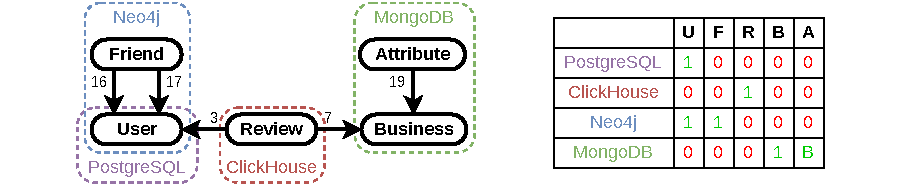
\includegraphics[width=\textwidth]{img/commentary-aimm_state.pdf}
    \caption{State representation from \Cref{ex:adapt-state}. Columns correspond to complex types and rows correspond to databases. The matrix captures model assignment, embedding, and cross-model redundancy.}
    \label{fig:adapt}
\end{figure}

\subsection{Search Strategy and Latency Estimation}

Even this finite state space is too large for exhaustive evaluation. We therefore explore it with \acrshort{mcts}. The algorithm incrementally builds a directed acyclic graph of evaluated states. It selects a promising path while balancing exploration and exploitation, expands the selected state by applying a migration step, evaluates the resulting configuration, and propagates the value back through the graph. A graph is needed instead of a tree because the same configuration may be reached through different sequences of operations.

The main difficulty is evaluating a configuration without materializing it. We use learned latency estimators based on query-plan information. The same idea can be extended to cross-model queries by combining the estimated costs of their subqueries and intermediate results. We also estimate migration and maintenance costs by modeling the database operations required to reach and preserve a configuration. The estimates are necessarily approximate, but they make systematic search feasible.

\subsection{Contributions}

Existing physical-design methods such as index and materialized-view selection optimize structures within a fixed logical representation~\citep{10.1145/3183713.3199671}. Learned tuning methods use workload behavior to predict latency or select system structures~\citep{10.14778/3342263.3342646, 10.1155/2023/8835111, 10.1007/s10844-022-00762-0}, but usually optimize an existing configuration rather than alternative mappings of one conceptual schema. Polystore and multistore systems address interoperation across backends~\citep{alotaibi2020estocada, DBLP:journals/ijcc/BondiombouyV16, 10.1145/3417990.3421999}, while migration approaches such as Darwin and MigCast focus on schema modification and migration~\citep{storl2022darwin, hillenbrand2019migcast}. Our contribution is to make the logical representation itself part of the optimization problem.

We defined a finite state space that captures model assignment, embedding, and cross-model redundancy. The categorical representation makes it possible to describe queries independently of the configurations, define transitions through schema modification operations, and migrate data to a selected configuration. This connects the search process to the same semantic framework used for modeling, querying, and evolution.

On top of this representation, we introduced an automated search process based on weighted workloads and \acrshort{mcts}. We implemented the approach in MM-mapsearch, including learned latency prediction, estimation of cross-model query costs, and an interactive interface for inspecting alternative configurations~\paperRef{edbt_2026}. This establishes a path from reactive evolution to proactive adaptation: the system can use workload observations to identify a better representation and evaluate whether its expected benefit justifies migration and maintenance costs.

%\endgroup
%\begingroup Complementary Approaches

\section{Complementary Approaches to Multi-Model Data Management}

The following approaches complement the main framework. Benchmarking provides the datasets and workloads needed to evaluate modeling, querying, evolution, and self-adaptation, while schema-free query unification addresses environments in which a shared conceptual schema is not yet available.

\subsection{Benchmarking \& Evaluation}

Our modeling and optimization techniques require datasets and workloads that cover many kinds, alternative model combinations, complex cross-model queries, and multiple versions of a schema. Existing benchmarks are mostly single-model: TPC-H~\citep{tpch} and TPC-DS~\citep{tpcds} target relational workloads, XMark~\citep{10.5555/1287369.1287455} and DeepBench~\citep{10.1145/3531348.3532176} target hierarchical or document data, and LDBC-SNB~\citep{10.1145/2723372.2742786} targets graph workloads. Multi-model benchmarks such as BigBench~\citep{10.1145/2463676.2463712}, UniBench~\citep{unibench}, and M2Bench~\citep{10.14778/3574245.3574259} are important steps, but they generally provide only a small number of kinds and relatively simple queries, and usually describe one fixed schema and workload. They are therefore not sufficient for evaluating the large configuration spaces and evolution scenarios considered here.

Generating a synthetic dataset from scratch is time-consuming and often produces data that is not realistic enough. Transforming an existing dataset usually requires a new custom script for each target representation. Such scripts are difficult to reuse and validate semantically. Our approach, proposed in \paperRef{enase_2025} and extended in~\citep{is_2026} (accepted after the thesis was submitted), uses the categorical framework to automate this process. \paperRef{edbt_2025} describes the implementation called \term{TransforMMer}.

The first step is to infer conceptual and logical schemas and the mappings between them~\citep{mm_infer, koupil2022mminfer}. Because some semantic decisions cannot be recovered from the data alone, users then refine the inferred schema by confirming references, adding missing identifiers, or unifying structurally similar fragments. We restrict this refinement to light operations, which keeps the mappings consistent with the original logical schema.

Users can then select one or more target logical representations. TransforMMer transforms the data through the instance category and produces semantically equivalent relational, document, graph, wide-column, or other supported representations. The process and its alternative outputs are illustrated in \Cref{fig:transformmer-sc}.

\begin{example}
\label{ex:transformmer-sc}
Starting with the Yelp dataset from \Cref{ex:mm-data}, TransforMMer infers a conceptual schema and mappings from the existing data. Users can confirm reference candidates and refine the schema, after which the system generates several semantically equivalent representations, such as two relational schemas with different degrees of embedding and a document schema with nested attributes. The resulting benchmark variants are shown in \Cref{fig:transformmer-sc}.
\end{example}

\begin{figure}[ht]
    \centering
    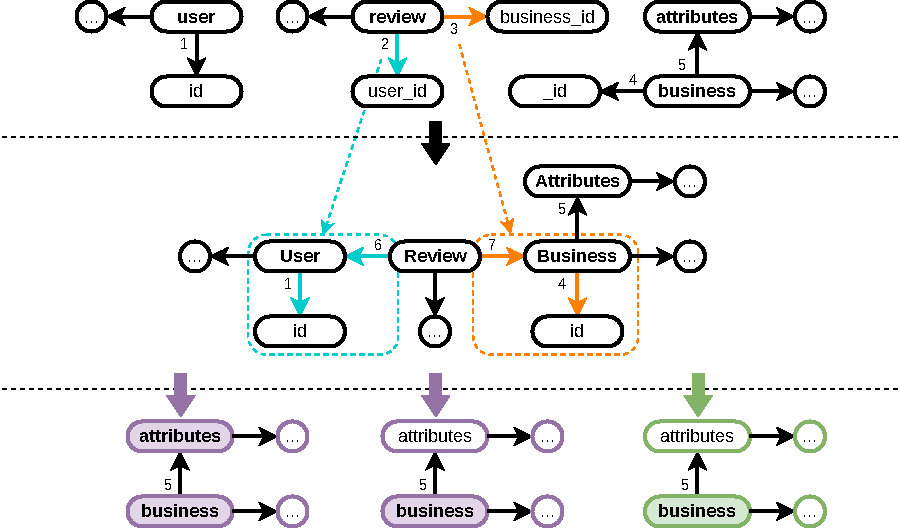
\includegraphics[width=\textwidth]{img/commentary-transformmer_sc.pdf}
    \caption{Benchmark creation from \Cref{ex:transformmer-sc}: inferred and refined conceptual schemas followed by several alternative logical representations.}
    \label{fig:transformmer-sc}
\end{figure}

The same framework supports benchmark evolution. Users can apply \acrshort{smo}s to create several versions of the conceptual schema; the system propagates the changes to the logical schemas and data so that all representations remain semantically aligned. Queries are defined in \acrshort{mmql} and evolved together with the schema. The query engine then generates comparable plans for the selected representations without executing them.

This changes the role of a benchmark. It is not merely a fixed dataset with a fixed workload, but a family of related data and workload variants that can expose how a system behaves under different representations and successive schema changes. Such a benchmark can evaluate querying, evolution, and self-adaptation within one controlled process.

\subsection{Schema-free Query Unification}

The categorical framework assumes an explicit conceptual schema and mappings. In highly dynamic settings such as data lakes, browser-side integration, or loosely coupled services, constructing this model before querying may be too costly or premature~\citep{CSUR-Jiaheng,AWSDataLake}. In these cases, users still need to combine heterogeneous data and query languages. We address this problem in \paperRef{vldb_2025_dortdb} with \term{DortDB}.

Rather than introducing another universal user language, DortDB preserves established languages. \acrshort{sql}~\citep{SQL}, XQuery~\citep{XQuery}, and Cypher~\citep{Cypher} can be nested recursively into one another, without imposing a privileged top-level language. The mixed query is translated into a \term{unified algebra} covering relational, hierarchical, and graph-style operators~\citep{DBLP:conf/icde/ReSF06, DBLP:conf/edbt/AnglesBGV25, DBLP:conf/sigmod/HolschGS16}. This algebra acts as a common compilation target, so the system can inspect, optimize, and execute the mixed query as one plan.

\Cref{ex:dortdb} illustrates the approach. Different parts of a cross-model query may use different languages, and the system switches between them at any point using a language marker. It then derives a single algebraic plan instead of treating nested queries as opaque calls.

\begin{example}
\label{ex:dortdb}
This query expresses the same task as \Cref{ex:query-multi}. Here, the outer query uses Cypher to match and filter reviews, while the nested \acrshort{sql} query retrieves the corresponding user.
\begin{alltt}\small\ttfamily
\cypher{MATCH} (review:Review)
\cypher{WHERE} review.business_id = 'bus#679' \cypher{AND} review.stars >= 3
\cypher{UNWIND} (
    \keyword{LANG sql}
    \sql{SELECT} user.id, user.name
    \sql{FROM} user
    \sql{WHERE} user.id = review.user_id
) \cypher{AS} u
\cypher{RETURN} review.stars \cypher{AS} stars, u.name \cypher{AS} name
\cypher{ORDER BY} stars \cypher{ASC}
\end{alltt}
The \term{LANG} keyword switches languages inside the query. DortDB translates the complete query into the unified algebra, where the relational and graph-style operations can be inspected and optimized together.
\end{example}

DortDB is not a replacement for the categorical framework. The schema-first approach provides stronger semantic guarantees, explicit mappings, evolution machinery, and reasoning about alternative representations. DortDB starts with existing heterogeneous sources and focuses on rapid interoperability with minimal setup. Its prototype is intentionally in-memory and read-only, which allows us to focus on language interoperability and optimization while leaving storage and transaction management aside.

\subsection{Contributions to Evaluation and Interoperability}

TransforMMer contributes a transformation-driven approach to benchmark engineering. It derives families of semantically aligned multi-model datasets, logical representations, and workloads from existing data. Because the process records the conceptual changes and transformations, it supports reproducible evaluation across model combinations and evolution steps~\paperRef{enase_2025, edbt_2025}. It also allows the same queries to be regenerated for each logical representation and schema version, making performance comparisons and evolution experiments directly comparable.

DortDB contributes a lightweight route to cross-model querying when an explicit schema is unavailable. Its unified algebra allows established query languages to interoperate symmetrically and provides a common basis for optimization (\paperRef{vldb_2025_dortdb}).

These two approaches address different prerequisites: TransforMMer supports systematic evaluation once semantic structure is available, whereas DortDB supports immediate querying when constructing that structure is not yet practical.

%\endgroup
%\begingroup Conclusion

\section{Conclusion}

We address multi-model data management as one problem spanning conceptual modeling, schema inference, transformation, querying, evolution, and workload-driven adaptation. The central idea is to use a shared conceptual representation as a stable semantic layer, without erasing the differences between the logical models and database systems that realize it.

The main contributions of this thesis are as follows:
\begin{itemize}
    \item \emph{Evolution} We defined atomic, composite, and complex schema modification operations and showed how they can be propagated through conceptual schemas, logical schemas, data, and queries. We also analyzed how schema changes affect existing queries and distinguished among valid queries, safe rewrites, approximate repairs, and cases that require additional user input. This allows the system to remain correct under schema evolution while using semantic evidence, including functional dependencies, to guide ambiguous decisions.
    \item \emph{Self-adaptation.} We formulated workload-aware adaptation as a search over alternative logical configurations, where the objective is to choose a representation that matches the workload while accounting for migration and maintenance cost. The resulting approach uses a finite state space and \acrshort{mcts}-based optimization to identify better representations without exhaustively benchmarking every alternative.
    \item \emph{Benchmarking.} We developed TransforMMer, which derives semantically aligned multi-model datasets, representations, and evolving workloads from existing data. This makes it possible to evaluate models, queries, and evolution scenarios under realistic and reproducible conditions.
    \item \emph{Schema-free query unification.} We developed DortDB as a complementary route to heterogeneous querying when a shared conceptual schema is not yet available. By preserving established query languages and translating mixed queries into a shared algebra, the approach supports practical interoperability without requiring a full semantic model upfront.
\end{itemize}

Overall, the thesis demonstrates that multi-model data management should be treated as one integrated problem rather than as a collection of isolated techniques. The conceptual schema remains the semantic anchor, schema evolution and query synchronization protect correctness, self-adaptation improves the representation when the workload changes, and schema-free interoperability extends the approach to dynamic settings. Together, these contributions provide a coherent framework for modeling, querying, evolving, and adapting multi-model data in practice.

%\endgroup
